\documentclass[iop]{emulateapj}
%\documentclass[12pt,preprint]{aastex}

\usepackage{epstopdf}
\usepackage{apjfonts,graphicx}
\usepackage{epsf}
\usepackage{hyperref}
\usepackage{url}
\usepackage[flushleft]{threeparttable}
%\usepackage{mathtools}

\newcommand{\kms}{\hbox{km~s$^{-1}$}}
\newcommand{\mas}{mas yr$^{-1}$}
\newcommand{\msun}{$M_{\odot}$}
\newcommand{\rsun}{$R_{\odot}$}

\begin{document}

\slugcomment{To be submitted to ApJ}
\shortauthors{Gnedin and Brown}
\shorttitle{HVS}

\title{Constraints on the Shape of the Galactic Halo from Accurate Measurements of Proper Motion of Hypervelocity Stars}
        
\author{Oleg Y.\ Gnedin\altaffilmark{1}, Warren R.\ Brown\altaffilmark{2}}

\altaffiltext{1}{Department of Astronomy, University of Michigan, Ann Arbor, MI 48109, USA}
\altaffiltext{2}{Smithsonian Astrophysical Observatory, 60 Garden St, Cambridge, MA 02138, USA}

\date{\today}

\begin{abstract}
We present predictions for a future astrometric mission...
\end{abstract}

\keywords{stars: early-type --- Galaxy: halo --- Galaxy: kinematics and dynamics}

\section{Introduction}

%para 1: HVS move fast and trace the Galactic potential from very small to very large scales

Hypervelocity stars (HVSs) are unbound stars ejected from the Galaxy by the 
Milky Way's central massive black hole (MBH) \citep{hills88, brown15}.  First 
discovered by \citet{brown05}, there are now 21 unbound main sequence B-type stars 
whose properties are best explained by this origin \citep{brown14}.  HVSs 
importantly connect the center of the Milky Way to the outer halo.  Launched on 
radial trajectories from the Galactic center, HVSs integrate the gravitational 
potential of the Milky Way as they travel to 100 kpc distances.

%para 2: This can be used to constrain the shape of the dark matter halo, because of tangential deflection

DM discussion.  

%para 3: Halo triaxiality is a robust prediction of CDM, least affected by the baryon effects

...If the mass distribution of the Milky Way is non-spherical, the 
trajectories of the HVSs must deviate from being precisely radial...

%para 4 or a section: What's new on HVS: we assume some chosen HVS come from the Galactic center for these several lines of evidence; caveats about alternative ejection scenarios; discuss why the unlikely ones are not chosen

There are now many lines of evidence to support the Galactic center origin 
of HVSs.  Following the first discovery, \citet{brown07b, brown14} performed a 
complete spectroscopic survey of halo stars with the colors of 3 \msun\ stars.  The 
color-selected survey found 21 stars unbound in radial velocity alone, plus a 
comparable number of outliers with bound velocities.  The bound and unbound velocity 
outliers all move outwards, consistent with an ejection origin, and the distribution 
of velocities is consistent with expectations from the Hills mechanism 
\citep{kenyon08, kenyon14}.  The number of unbound B-type stars is also consistent 
with theoretically predicted ejection rates \citep{hills88, zhang10, zhang13}.  
Follow-up echelle observations establish that the unbound stars are rapid rotators 
$55 < v\sin{i} < 320$ \kms\ and thus main-sequence B stars \citep{przybilla08b, 
lopezmorales08, brown12c, brown13b}.  The difference between their estimated ages 
and flight times is 100 Myr, a timescale inconsistent with scenarios that require 
prompt ejection, such as supernovae, but consistent with a Galactic center origin 
\citep{brown12c}.  While extreme supernova ejections can overlap in velocity with 
HVSs \citep{heber08}, high velocity ejections from the disk will have a strong 
Galactic latitude dependence because of the rotation of the disk \citep{bromley09}.  
Observed unbound B stars are spread uniformly over Galactic latitude, inconsistent 
with a disk origin but consistent with a Galactic center origin \citep{brown12b}.  
The Milky Way's MBH must eject HVSs, and only the MBH ejection can self-consistently 
explain the the number, velocity, stellar nature, flight time, and spatial 
distribution of the observed unbound B stars.

Further evidence for the Galactic center origin of HVSs is found in the 
Galactic center.  Several dozen B-type stars orbit within about 0.04 pc of the MBH 
on randomly orientated, eccentric orbits (the so-called S stars) \citep{ghez08, 
gillessen09}.  Spectroscopy establishes that the S stars are normal main-sequence B 
stars \citep{ghez03, eisenhauer05}.  The tidal forces of the MBH are too strong to 
permit star formation in these close orbits \citep{morris93}, thus the short-lived B 
must form elsewhere and then be captured next to the MBH \citep{gould03}.

The same three-body exchange that ejects a HVS also captures a star onto an 
tight, eccentric orbit around the MBH, thus the S stars are the likely former 
companions of HVSs.  The number of S stars is consistent with the number of unbound 
B stars in the halo \citep{bromley12, kenyon14}.  The distribution of S star 
eccentricities matches predictions of the Hills mechanism \citep{perets09c, zhang13, 
madigan14}.  Stars at larger radii from the MBH have increasingly eccentric orbits, 
consistent with their being captured by the Hills mechanism onto orbits with longer 
relaxation times \citep{madigan14}.  Thus the number, orbital distribution, and 
stellar nature of stars orbiting the central MBH supports the HVS ejection 
mechanism.


\begin{center}
\begin{deluxetable*}{cccccc}
\tabletypesize{\footnotesize}
\tablewidth{0pt}
\tablecaption{UNBOUND HYPERVELOCITY STARS\label{tab:hvs}}
\tablecolumns{6}
\tablehead{
	\colhead{ID} &
	\colhead{RA, Dec} & 
	\colhead{$g_0$} & 
	\colhead{$d_{\rm helio}$} &
	\colhead{$v_{\rm helio}$} & 
	\colhead{$\mu_{\rm RA}, \mu_{\rm Dec}$} \\
          & (J2000) & (mag) & (kpc) & (\kms) & (\mas)
        }
\startdata
HVS 1  &  9:07:44.99, $+$02:45:06.9 & $19.69\pm0.023$ & $102\pm15 $ & $831.1\pm 5.7$ & $+0.08\pm0.26$, $-0.12\pm0.22$ \\
HVS 4  &  9:13:01.00, $+$30:51:19.9 & $18.34\pm0.023$ & $ 64\pm9.8$ & $600.9\pm 6.2$ & $-0.23\pm0.36$, $-0.42\pm0.36$ \\
HVS 5  &  9:17:59.47, $+$67:22:38.3 & $17.58\pm0.032$ & $ 45\pm5.2$ & $545.5\pm 4.3$ & $+0.55\pm0.61$, $-0.44\pm0.59$ \\
HVS 6  & 11:05:57.45, $+$09:34:39.4 & $18.94\pm0.024$ & $ 55\pm6.9$ & $609.4\pm 6.8$ & $+0.05\pm0.57$, $+0.31\pm0.97$ \\
HVS 7  & 11:33:12.13, $+$01:08:24.8 & $17.63\pm0.015$ & $ 52\pm6.4$ & $526.9\pm 3.0$ & $+1.00\pm0.82$, $-0.55\pm1.04$ \\
HVS 8  &  9:42:14.03, $+$20:03:22.0 & $17.93\pm0.016$ & $ 53\pm9.8$ & $499.3\pm 2.9$ & $-0.82\pm1.16$, $-0.04\pm0.49$ \\
HVS 9  & 10:21:37.08, $-$00:52:34.7 & $18.64\pm0.023$ & $ 74\pm12 $ & $616.8\pm 5.1$ & $-1.26\pm0.74$, $-0.25\pm0.70$ \\
HVS 10 & 12:03:37.85, $+$18:02:50.3 & $19.24\pm0.024$ & $ 52\pm5.8$ & $467.9\pm 5.6$ & $-1.07\pm0.36$, $-0.58\pm0.42$ \\
HVS 12 & 10:50:09.60, $+$03:15:50.6 & $19.63\pm0.024$ & $ 66\pm8.5$ & $552.2\pm 6.6$ & $-0.40\pm0.36$, $+0.31\pm0.34$ \\
HVS 13 & 10:52:48.31, $-$00:01:33.9 & $20.01\pm0.021$ & $105\pm19 $ & $569.3\pm 6.1$ & $-0.90\pm0.38$, $+0.46\pm0.44$ \\
HVS 14 & 10:44:01.75, $+$06:11:39.0 & $19.72\pm0.023$ & $102\pm16 $ & $537.3\pm 7.2$ &       \nodata ,       \nodata  \\
HVS 15 & 11:33:41.09, $-$01:21:14.2 & $19.15\pm0.020$ & $ 66\pm9.6$ & $461.0\pm 6.3$ &       \nodata ,       \nodata  \\
HVS 16 & 12:25:23.40, $+$05:22:33.8 & $19.33\pm0.029$ & $ 71\pm12 $ & $429.8\pm 7.0$ &       \nodata ,       \nodata  \\
HVS 17 & 16:41:56.39, $+$47:23:46.1 & $17.43\pm0.015$ & $ 50\pm4.4$ & $250.2\pm 2.9$ &       \nodata ,       \nodata  \\
HVS 18 & 23:29:04.95, $+$33:00:11.4 & $19.30\pm0.015$ & $ 77\pm11 $ & $237.3\pm 6.4$ &       \nodata ,       \nodata  \\
HVS 19 & 11:35:17.76, $+$08:02:01.4 & $20.06\pm0.035$ & $ 97\pm15 $ & $592.8\pm11.8$ &       \nodata ,       \nodata  \\
HVS 20 & 11:36:37.13, $+$03:31:06.8 & $19.81\pm0.025$ & $ 75\pm11 $ & $512.1\pm 8.5$ &       \nodata ,       \nodata  \\
HVS 21 & 10:34:18.25, $+$48:11:34.5 & $19.73\pm0.030$ & $108\pm21 $ & $356.8\pm 7.5$ &       \nodata ,       \nodata  \\
HVS 22 & 11:41:46.45, $+$04:42:17.2 & $20.18\pm0.042$ & $ 84\pm13 $ & $597.8\pm13.4$ &       \nodata ,       \nodata  \\
HVS 23 & 21:56:29.02, $+$00:54:44.1 & $20.20\pm0.027$ & $115\pm20 $ & $259.3\pm 9.8$ &       \nodata ,       \nodata  \\
HVS 24 & 11:11:36.44, $+$00:58:56.4 & $18.86\pm0.016$ & $ 54\pm7.5$ & $492.5\pm 5.3$ &       \nodata ,       \nodata  
\enddata
\end{deluxetable*}
\end{center}
~\vspace{2.2cm}


\section{What affects the expected tangential motion}

\subsection{Flattening of stellar distribution}

\subsection{Halo triaxiality}

Fig 1: Cartoon of proper motions for two different orientations of dark matter halo (prolate vs. oblate) that match the observed vlos and position, to illustrate figure 2

\subsection{New fit to mass model}

\begin{figure}[t]
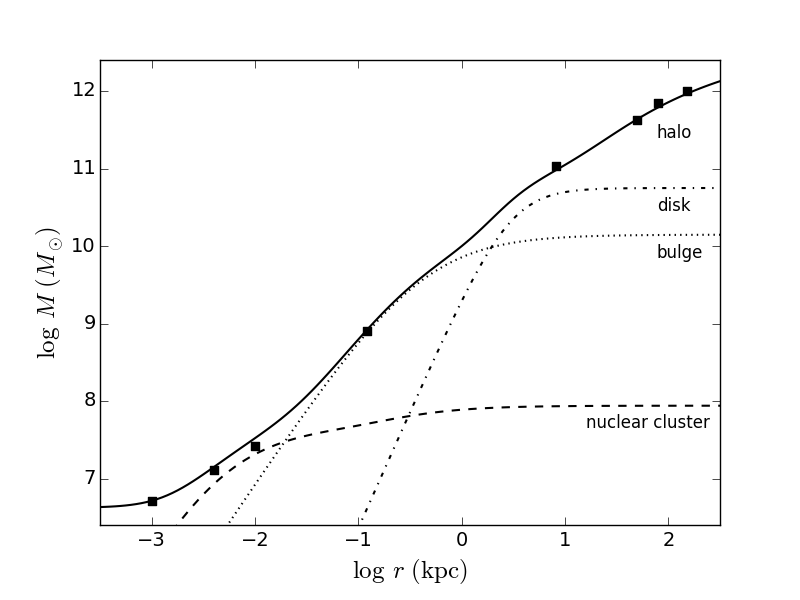
\includegraphics[width=1.05\hsize]{galactic_mass_obs.png}
  \vspace{-0.2cm}
\caption{\small New model of mass distribution in the Galaxy.}
  \vspace{0.3cm}
  \label{fig:galactic_model}
\end{figure}

Fig 2: mass distribution in the adopted Galactic model with existing observations



\section{Expected proper motion}

calculate expected proper motion for different orientation of the triaxial halo

\begin{figure}[t]
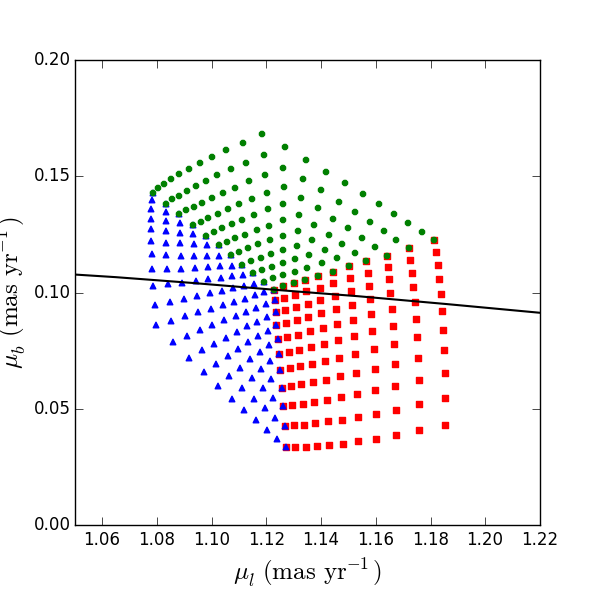
\includegraphics[width=1.05\hsize]{pm_hvs5.png}
  \vspace{-0.2cm}
\caption{\small Spread of expected proper motions for different configurations of the triaxial dark matter halo.}
  \vspace{0.3cm}
  \label{fig:pm_hvs5}
\end{figure}

Fig 3: Spread of proper motion for one star

%\begin{figure}[t]
%\includegraphics[width=1.05\hsize]{pm_hvs5_diff.png}
%  \vspace{-0.2cm}
%\caption{\small Difference in expected proper motions for different %ejection location within the Galactic disk.}
%  \vspace{0.3cm}
%  \label{fig:pm_hvs5_diff}
%\end{figure}

\begin{figure*}[t]
  \begin{minipage}{\hsize}
    \centering
    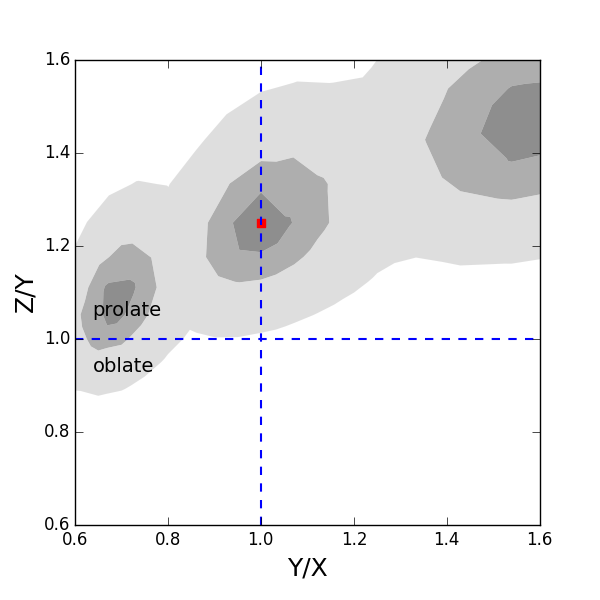
\includegraphics[width=3.4in]{axis_hvs5_nod.png}
    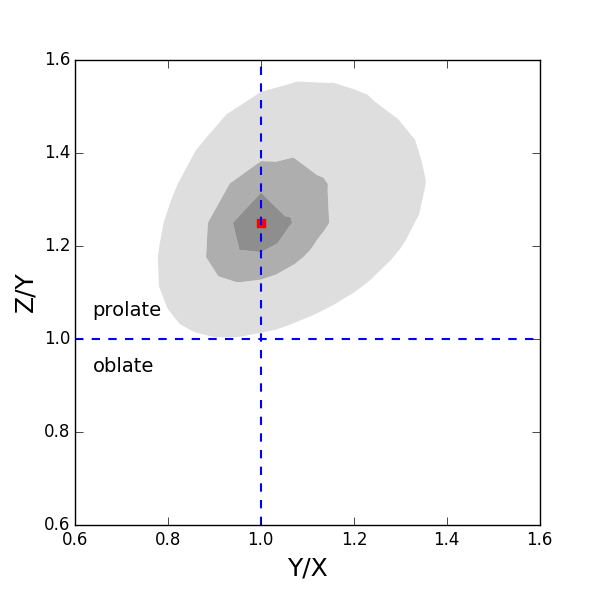
\includegraphics[width=3.4in]{axis_hvs5_d20.png}
  \end{minipage}
  \vspace{-0.2cm}
\caption{\small Constraints on axis ratios of the triaxial dark matter halo for one star with ({\it right panel}) and without ({\it left panel}) distance information.}
  \vspace{0.3cm}
  \label{fig:axis_hvs5}
\end{figure*}

Fig 4: Constraints on axis ratios without and with distance information (20\% distance error) for one star (HVS 5)

\begin{figure*}[t]
  \begin{minipage}{\hsize}
    \centering
    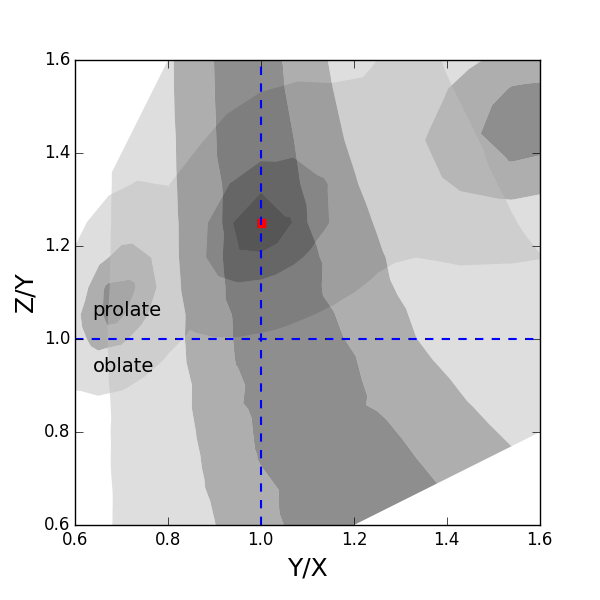
\includegraphics[width=3.4in]{axis_hvs5_9_nod.png}
    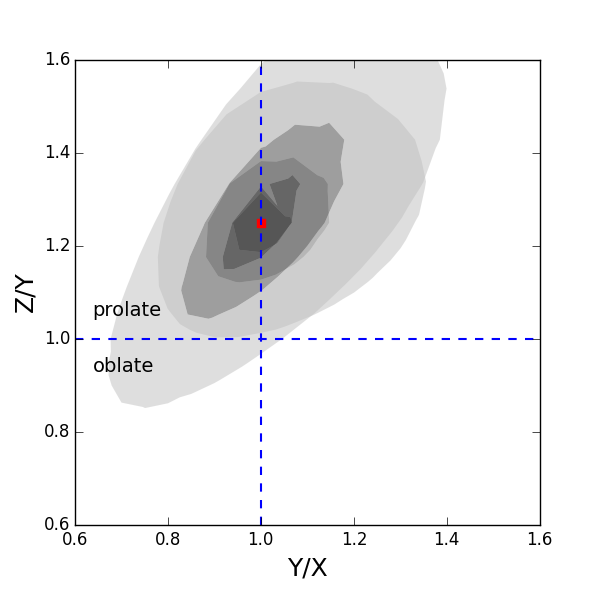
\includegraphics[width=3.4in]{axis_hvs5_9_d20.png}
  \end{minipage}
  \vspace{-0.2cm}
\caption{\small Constraints on axis ratios of the triaxial dark matter halo for two stars with ({\it right panel}) and without ({\it left panel}) distance information.}
  \vspace{0.3cm}
  \label{fig:axis_hvs5_9}
\end{figure*}

Fig 5: Same for overlapping contours of two stars (HVS 5 and 4 or 9)

and/or Fig 6: Same for central bands (tiny p.m. error) for all stars, to illustrate which stars are best and what can be gained from a larger sample

OLEG TO DO: quantitative way to combine several measurements expected from Gaia; write down full likelihood; check if joint constraints could be tighter than naive overlap of contours


\section{Discussion}

Gaia Data Release 2 at the end of 2017 will have too large uncertainty

argue for future space-based astrometric mission with large FOV to include enough quasars and reach high enough accuracy of p.m.

complementary probes of halo shape; current constraints are consistent with spherical

and at larger distances than tidal streams


\section{Conclusion}\label{sec:pm}

test of dark matter physics

robust test of CDM model predictions

requires future, more accurate mission to do it


\section{Summary}\label{sec:sum}

We 


\bigskip
\acknowledgements

This research makes use of SAO/NASA's Astrophysics Data System Bibliographic Services.  This work was supported in part by the Smithsonian Institution. ....
O.G. was supported in part by NASA through grant NNX12AG44G, and by NSF through grant AST-1412144.

\makeatletter\@chicagotrue\makeatother

\bibliographystyle{apj}
%\bibliography{gc}

\begin{thebibliography}{25}
\expandafter\ifx\csname natexlab\endcsname\relax\def\natexlab#1{#1}\fi

\bibitem[{{Bromley} {et~al.}(2009){Bromley}, {Brown}, {Geller}, \&
  {Kenyon}}]{bromley09}
{Bromley}, B.~C., {Brown}, W.~R., {Geller}, M.~J., \& {Kenyon}, S.~J. 2009,
  \apj, 706, 925

\bibitem[{{Bromley} {et~al.}(2012){Bromley}, {Kenyon}, {Geller}, \&
  {Brown}}]{bromley12}
{Bromley}, B.~C., {Kenyon}, S.~J., {Geller}, M.~J., \& {Brown}, W.~R. 2012,
  \apjl, 749, L42

\bibitem[{{Brown}(2015)}]{brown15}
{Brown}, W.~R. 2015, \araa, 53, 15

\bibitem[{{Brown} {et~al.}(2012{\natexlab{a}}){Brown}, {Cohen}, {Geller}, \&
  {Kenyon}}]{brown12c}
{Brown}, W.~R., {Cohen}, J.~G., {Geller}, M.~J., \& {Kenyon}, S.~J.
  2012{\natexlab{a}}, \apjl, 754, L2

\bibitem[{{Brown} {et~al.}(2013){Brown}, {Cohen}, {Geller}, \&
  {Kenyon}}]{brown13b}
---. 2013, \apj, 775, 32

\bibitem[{{Brown} {et~al.}(2012{\natexlab{b}}){Brown}, {Geller}, \&
  {Kenyon}}]{brown12b}
{Brown}, W.~R., {Geller}, M.~J., \& {Kenyon}, S.~J. 2012{\natexlab{b}}, \apj,
  751, 55

\bibitem[{{Brown} {et~al.}(2014){Brown}, {Geller}, \& {Kenyon}}]{brown14}
---. 2014, \apj, 787, 89

\bibitem[{{Brown} {et~al.}(2005){Brown}, {Geller}, {Kenyon}, \&
  {Kurtz}}]{brown05}
{Brown}, W.~R., {Geller}, M.~J., {Kenyon}, S.~J., \& {Kurtz}, M.~J. 2005,
  \apjl, 622, L33

\bibitem[{{Brown} {et~al.}(2007){Brown}, {Geller}, {Kenyon}, {Kurtz}, \&
  {Bromley}}]{brown07b}
{Brown}, W.~R., {Geller}, M.~J., {Kenyon}, S.~J., {Kurtz}, M.~J., \& {Bromley},
  B.~C. 2007, \apj, 671, 1708

\bibitem[{{Eisenhauer} {et~al.}(2005){Eisenhauer}, {Genzel}, {Alexander},
  {et~al.}}]{eisenhauer05}
{Eisenhauer}, F., {Genzel}, R., {Alexander}, T., {et~al.} 2005, \apj, 628, 246

\bibitem[{{Ghez} {et~al.}(2008){Ghez}, {Salim}, {Weinberg}, {et~al.}}]{ghez08}
{Ghez}, A.~M., {Salim}, S., {Weinberg}, N.~N., {et~al.} 2008, \apj, 689, 1044

\bibitem[{{Ghez} {et~al.}(2003)}]{ghez03}
{Ghez}, A.~M. {et~al.} 2003, \apjl, 586, L127

\bibitem[{{Gillessen} {et~al.}(2009){Gillessen}, {Eisenhauer}, {Trippe},
  {et~al.}}]{gillessen09}
{Gillessen}, S., {Eisenhauer}, F., {Trippe}, S., {et~al.} 2009, \apj, 692, 1075

\bibitem[{{Gould}(2003)}]{gould03}
{Gould}, A. 2003, \apjl, 592, L63

\bibitem[{{Heber} {et~al.}(2008){Heber}, {Edelmann}, {Napiwotzki}, {Altmann},
  \& {Scholz}}]{heber08}
{Heber}, U., {Edelmann}, H., {Napiwotzki}, R., {Altmann}, M., \& {Scholz},
  R.-D. 2008, \aap, 483, L21

\bibitem[{{Hills}(1988)}]{hills88}
{Hills}, J.~G. 1988, \nat, 331, 687

\bibitem[{{Kenyon} {et~al.}(2014){Kenyon}, {Bromley}, {Brown}, \&
  {Geller}}]{kenyon14}
{Kenyon}, S.~J., {Bromley}, B.~C., {Brown}, W.~R., \& {Geller}, M.~J. 2014,
  \apj, 793, 122

\bibitem[{{Kenyon} {et~al.}(2008){Kenyon}, {Bromley}, {Geller}, \&
  {Brown}}]{kenyon08}
{Kenyon}, S.~J., {Bromley}, B.~C., {Geller}, M.~J., \& {Brown}, W.~R. 2008,
  \apj, 680, 312

\bibitem[{{L{\'o}pez-Morales} \& {Bonanos}(2008)}]{lopezmorales08}
{L{\'o}pez-Morales}, M. \& {Bonanos}, A.~Z. 2008, \apjl, 685, L47

\bibitem[{{Madigan} {et~al.}(2014){Madigan}, {Pfuhl}, {Levin},
  {et~al.}}]{madigan14}
{Madigan}, A.-M., {Pfuhl}, O., {Levin}, Y., {et~al.} 2014, \apj, 784, 23

\bibitem[{{Morris}(1993)}]{morris93}
{Morris}, M. 1993, \apj, 408, 496

\bibitem[{{Perets}(2009)}]{perets09c}
{Perets}, H.~B. 2009, \apj, 690, 795

\bibitem[{{Przybilla} {et~al.}(2008){Przybilla}, {Nieva}, {Tillich},
  {et~al.}}]{przybilla08b}
{Przybilla}, N., {Nieva}, M.~F., {Tillich}, A., {et~al.} 2008, \aap, 488, L51

\bibitem[{{Zhang} {et~al.}(2010){Zhang}, {Lu}, \& {Yu}}]{zhang10}
{Zhang}, F., {Lu}, Y., \& {Yu}, Q. 2010, \apj, 722, 1744

\bibitem[{{Zhang} {et~al.}(2013){Zhang}, {Lu}, \& {Yu}}]{zhang13}
---. 2013, \apj, 768, 153

\end{thebibliography}

\end{document}